\documentclass[12pt]{article}

\usepackage{algorithmic}
\usepackage{amsmath}
\usepackage{graphicx}
\usepackage{hyperref}
\usepackage{booktabs}

\begin{document}

\title{CSI709 Midterm \\
Problem 1}
\author{
        Geoffrey Ulman \\
        George Mason University\\
}
\date{\today}

\maketitle

\section{Results}

\begin{figure}
\centering
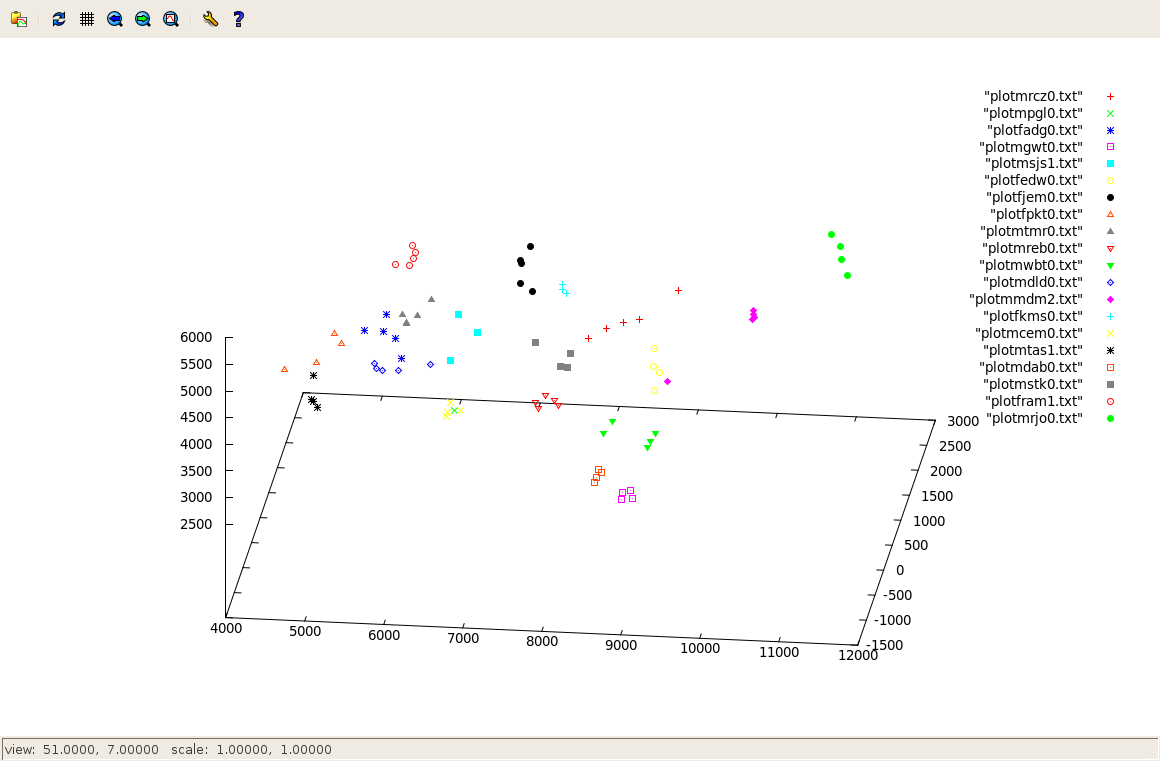
\includegraphics[width=0.30\textwidth]{pca-screen-1.png}
\caption{Faces Projected Into PCA Space Using First 3 Eigenfaces}
\label{pca1}
\end{figure}

\begin{figure}
\centering
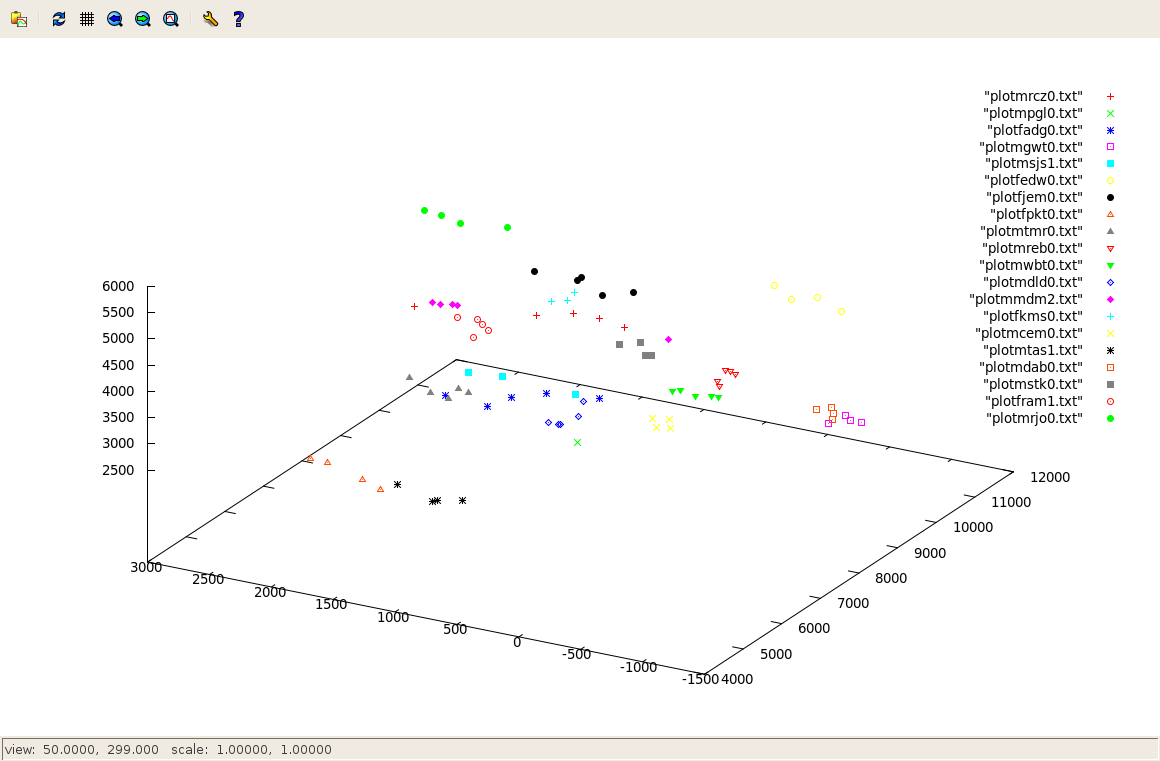
\includegraphics[width=0.30\textwidth]{pca-screen-2.png}
\caption{Rotated View}
\label{pca1}
\end{figure}

\end{document}
